\documentclass{article}

\usepackage{amsthm} % el de teoremas
\usepackage{amsmath} % ?
\usepackage{amssymb} % ?
\usepackage{mathtools} % \coloneq
\usepackage{csquotes} % no agregarlo genera un error con biblatex
\usepackage{biblatex}
\usepackage{listings}
\usepackage{graphicx}
\graphicspath{ {./images} }

\usepackage[spanish]{babel}
\usepackage{hyperref}

% defino mis teoremas
\newtheorem{theorem}{Theorem}
\newtheorem{corollary}{Corollary}[theorem]
\newtheorem{lemma}[theorem]{Lemma}

\theoremstyle{definition}
\newtheorem{definition}{Definition}

\renewcommand\qedsymbol{$\blacksquare$} % para que aparezca el cuadradito negro

\title{Sistemas\_Operativos - Assignment 3}
\author{Oscar Vargas Pabon}
\date{Mayo 2025}

\begin{document}
	\maketitle
	\tableofcontents
	
	El repositorio con el código desarrollado está en 
	
	 \url{https://github.com/osvarp/SO_ASS_3}.
\section{Review conceptual}
\subsection{a)}
	"Disk requests come into the disk driver for cylinders 10, 22,
	20, 2, 40, 6, and 38, in that order. A seek takes 6 msec per
	cylinder. How much seek time is needed for (a) First-come,
	first served. (b) Closest cylinder next. (c) Elevator
	algorithm (initially moving upward). In all cases, the arm is
	initially at cylinder 20."
	
	\textbf{FCFS: }
	Toma un tiempo de $146 (cilindro) \cdot 6 (\frac{msec}{cilindro}) = 876 (msec)$.
	
	\textbf{SSTF: }
	Toma un tiempo de $60 (cilindro) \cdot 6 (\frac{msec}{cilindro}) = 360 (msec)$.
	
	\textbf{Elevator: }
	Toma un tiempo de $58 (cilindro) \cdot 6 (\frac{msec}{cilindro}) = 348 (msec)$.

\subsection{b)}
	"Suppose that a disk drive has 5,000 cylinders, numbered 0 to
	4,999. The drive is currently serving a request at cylinder
	2,150, and the previous request was at cylinder 1,805. The
	queue of pending requests, in FIFO order, is: 2,069; 1,212;
	2,296; 2,800; 544; 1,618; 356; 1,523; 4,965; 3,681 Starting
	from the current head position, what is the total distance (in
	cylinders) that the disk arm moves to satisfy all the pending
	requests for each of the following disk-scheduling algorithms?
	a. FCFS b. SCAN c. C-SCAN"
	
	\textbf{FCFS: }
	Toma una distancia de 11,727 cilindros el completar todas las 'requests' pendientes.
	
	\textbf{SCAN: }
	Toma una distancia de 7,492 cilindros el completar todas las 'requests' pendientes.
	
	\textbf{C-SCAN: }
	Toma una distancia de 9,917 cilindros el completar todas las 'requests' pendientes.
	
\subsection{c)}
	"A slight modification of the elevator algorithm for scheduling
	disk requests is to always scan in the same direction. In what
	respect is this modified algorithm better than the elevator
	algorithm?"
	
	Es preferible en el sentido en el que hace que los tiempos de espera sean más uniformes. 

\section{Implementacion}
	Separe en 4 archivos la implementación.
	
	En 'dsk\_sched.py' implemente los algoritmos de scheduling. Cada uno de estos retorna el tiempo (medido en cilindros) y el orden en el que va a procesar los 'requests'. Los algoritmos implementados fueron: FCFS, SSTF, SCAN (comienza hacia arriba), C-SCAN (comienza hacia arriba). Notar que para SCAN y C-SCAN, en el orden de los 'requests' se incluyen los recorridos hasta los limites (0,limit).
	
	En 'generate\_cases.py' implemente el generador de casos pseudo-aleatorio.
	
	En 'visualizer.py' implemente las funciones relacionadas a la visualización de la salida.
	
	En 'main.py' implemente la interfaz con el usuario y las demás funciones.
	
\section{Visualizacion}
	La visualización del movimiento del brazo se realizo utilizando la libreria de
	matplotlib.pyplot. Un ejemplo de esta salida se encuentra en la figura 1.
	
	\begin{figure}
		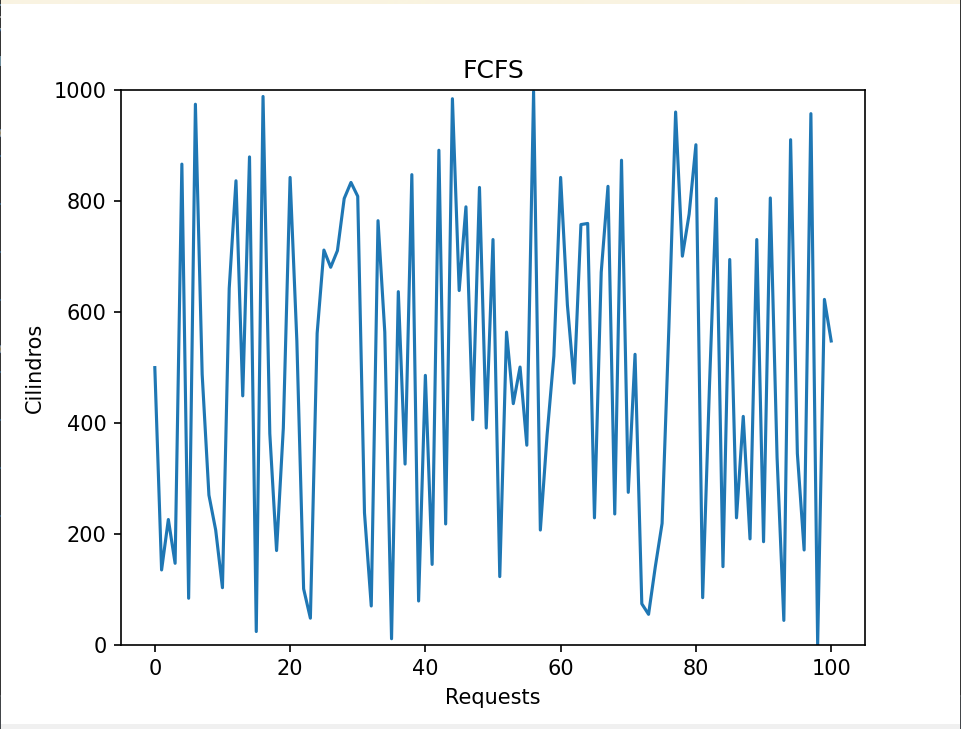
\includegraphics[width=1\linewidth]{FCFS_500_100_1000.png}
		\caption{Caso generado aleatoriamente. Inicia en 500, tiene 100 'requests' y tiene 1000 cilindros.}
	\end{figure}
	
	La visualización de los tiempos (medidos en cantidad de cilindros) que toman los algoritmos en resolver todas sus 'requests' se imprime en una tabla a stdout. Un ejemplo de esta salida se encuentra en la figura 2.
	
	\begin{figure}
		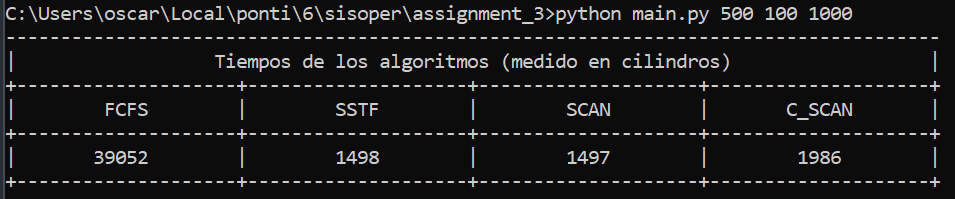
\includegraphics[width=1\linewidth]{tiempos_500_100_1000.png}
		\caption{Caso generado aleatoriamente. Inicia en 500, tiene 100 'requests' y tiene 1000 cilindros.}
	\end{figure}
	
	La entrada es recibida por 'main.py' mediante linea de comandos. El primer parametro es la poscicion inicial del brazo, el segundo la cantidad de 'requests' a generar, el tercero la cantidad total de cilindros del disco. Notar que de no especificar alguno de estos, tomara sus valores predeterminados: 0 para la poscicion inicial, 1000 para los 'requests', y 5000 para el total de cilindros.
	
	\[python \text{ } main.py \text{ } <strt> \text{ } <sz> \text{ } <limit>\]
	
\end{document}